\documentclass[11pt,a4paper]{article}
\usepackage[utf8]{inputenc}
\usepackage[T1]{fontenc}
\usepackage[margin=1in]{geometry}
\usepackage{graphicx}
\usepackage{hyperref}
\usepackage{xcolor}
\usepackage{float}
\usepackage{listings}
\usepackage{upquote}
\usepackage{amsmath}
\usepackage{enumitem}
\usepackage{tcolorbox}
\tcbuselibrary{skins}

% Code listing style
\lstset{
    basicstyle=\ttfamily\small,
    breaklines=true,
    breakatwhitespace=false,
    frame=single,
    numbers=left,
    numberstyle=\tiny,
    backgroundcolor=\color{gray!10},
    keywordstyle=\color{blue},
    commentstyle=\color{green!50!black},
    stringstyle=\color{red},
    showstringspaces=false
}

% Callout boxes
\newtcolorbox{notebox}{colback=blue!5,colframe=blue!40!black,title=Note,fonttitle=\bfseries}
\newtcolorbox{warnbox}{colback=orange!5,colframe=orange!60!black,title=Common Mistake,fonttitle=\bfseries}
\newtcolorbox{checklistbox}{colback=green!5,colframe=green!40!black,title=Before Moving On,fonttitle=\bfseries}

\title{\textbf{Practice 4 --- Half-Term Challenge: Grabbing an Object}}
\author{
    Robotics and Cyber-Physical Systems \\
    School of Sciences and Engineering \\
    Tecnol\'ogico de Monterrey
}
\date{}

\begin{document}

\maketitle

\section*{Introduction}

This is the half-term challenge. You will build a complete autonomous manipulation pipeline that combines everything covered so far: forward kinematics, 3D object localization, visual servoing, and multi-phase state machine control.

The goal is simple to describe: \emph{find a blue object, drive toward it, position the gripper, and pick it up}. But achieving this reliably requires coordinating multiple control loops, switching between cameras, and managing robot state safely.

\subsection*{How This Practice Works}

Rather than writing one large script, you build five progressively more capable scripts:

\begin{center}
\begin{tabular}{lll}
\hline
\textbf{Script} & \textbf{New capability added} & \textbf{Phases active} \\
\hline
\texttt{p4\_1\_locate\_object.py} & 3D localization and plotting & --- (stationary) \\
\texttt{p4\_2\_approach.py}       & Autonomous approach          & approach \\
\texttt{p4\_3\_align.py}          & Fine alignment               & approach → align \\
\texttt{p4\_4\_reach.py}          & Arm extension                & approach → align → reach \\
\texttt{p4\_5\_grab.py}           & Gripper close                & approach → align → reach → grab \\
\hline
\end{tabular}
\end{center}

Each script is a direct copy of the previous one with one new block of logic added. \textbf{Always verify each script works before building on it}---a bug in Part 2 will be much harder to diagnose after Part 4 layers code on top.

\subsection*{Before You Begin}

Update your repository and synchronize dependencies:

\begin{lstlisting}[language=bash]
git pull
git fetch origin
git reset --hard origin/main
uv sync
\end{lstlisting}

\subsubsection*{Simulator Starting Position}

The file \texttt{stretch\_toolkit/sim\_config.json} controls where the robot spawns in the simulator. If you have used this repository before, you may recognise it as the renamed \texttt{robocasa\_config.json}---it serves the same purpose but now includes additional settings such as the starting position.

\begin{lstlisting}[language=json]
{
  "start_translation": [0, 1.0, 0]
}
\end{lstlisting}

The values are \texttt{[x, y, z]} in metres. The blue object (on the table) is at $y \approx -1.0$, so increasing \texttt{y} moves the robot further away. The default \texttt{y = 1.0} places the robot about 2\,m from the table---a good starting distance for the approach phase. If the robot spawns too close or too far, adjust this value before running your scripts.

\textbf{Reference: key tools in \texttt{stretch\_toolkit}}

\begin{itemize}
    \item \texttt{RobotTransforms(controller)} --- runs forward kinematics on the current joint state to compute where each link and camera is in the world. Must be constructed before the loop.
    \item \texttt{locate\_object(centroid, depth\_cam, transforms)} --- given a pixel centroid from a depth camera, returns \texttt{(obj2cam\_T, obj2base\_T)}: the object's 4×4 homogeneous pose in camera frame and robot base frame. The position in meters is the last column: \texttt{T[0:3, 3]}.
    \item \texttt{ObjectPlotter()} --- opens a live 3D matplotlib window. Call \texttt{plotter.update(cam\_T, obj\_T)} each loop tick. Pass \texttt{None} for \texttt{obj\_T} when no object is detected. Call \texttt{plotter.close()} in the \texttt{finally} block.
    \item \texttt{StateController(controller, targets)} --- a proportional controller that drives a set of joints to target positions. \texttt{get\_command()} returns velocity commands each tick. \texttt{is\_at\_goal()} returns \texttt{True} once all joints are within tolerance.
    \item \texttt{merge\_proportional(primary, secondary)} --- blends two velocity dictionaries. The \texttt{primary} (manual teleop) takes priority when non-zero; \texttt{secondary} (autonomous) fills in otherwise.
    \item \texttt{HEAD\_CAMERA}, \texttt{WRIST\_CAMERA} --- depth camera info objects (used by \texttt{locate\_object} and \texttt{.get\_depth()}).
    \item \texttt{HEAD\_RGB\_CAMERA}, \texttt{WRIST\_RGB\_CAMERA} --- RGB camera objects. Call \texttt{.get\_frame()} to get the current image as a NumPy array. Always check for \texttt{None} before use.
\end{itemize}

\subsection*{The Main Loop Pattern}

Every script in this practice follows the same main loop structure. The pattern below is your template---write all your per-phase logic inside the loop:

\begin{lstlisting}[language=Python]
while True:
    velocities = teleop.get_normalized_velocities()  # manual override input
    auto_velocities = {}                              # autonomous commands go here

    # --- your logic: populate auto_velocities based on sensor readings ---

    velocities = merge_proportional(velocities, auto_velocities)
    controller.set_velocities(velocities)
    cv2.waitKey(1)
    time.sleep(1 / 30)  # 30 Hz
\end{lstlisting}

\begin{notebox}
\texttt{merge\_proportional} is called \emph{after} your logic populates \texttt{auto\_velocities}. Do not call \texttt{controller.set\_velocities} inside individual phase branches---call it once at the bottom of the loop.
\end{notebox}

\newpage

\section*{Part 1 --- Object Localization and 3D Visualization}

\subsection*{Objective}

Detect a blue object using HSV color segmentation, compute its 3D position in the robot's base frame, and visualize it in a live 3D plot. This is the perception foundation the later phases depend on.

\subsection*{Task}

Create \texttt{p4\_1\_locate\_object.py} from the boilerplate with these imports:

\begin{lstlisting}[language=Python]
from stretch_toolkit import (
    controller, teleop, merge_proportional, locate_object,
    BACKEND_NAME, HEAD_CAMERA, HEAD_RGB_CAMERA,
    RobotTransforms, ObjectPlotter
)
import time
import cv2
import numpy as np

print(f"\n=== Running on {BACKEND_NAME} backend ===\n")
\end{lstlisting}

\subsubsection*{Step 1: Write the Object Detection Function}

Add this function \emph{above} \texttt{main()}. It converts the image to HSV, creates a binary mask for blue pixels, finds contours, and returns the centroid of the largest one:

\begin{lstlisting}[language=Python]
def find_blue_object(rgb_frame):
    if rgb_frame is None:
        return None
    hsv = cv2.cvtColor(rgb_frame, cv2.COLOR_BGR2HSV)
    mask = cv2.inRange(hsv,
                       np.array([110, 100, 100]),
                       np.array([130, 255, 255]))
    contours, _ = cv2.findContours(mask, cv2.RETR_EXTERNAL,
                                   cv2.CHAIN_APPROX_SIMPLE)
    if contours:
        largest = max(contours, key=cv2.contourArea)
        M = cv2.moments(largest)
        if M['m00'] > 0:
            cx = int(M['m10'] / M['m00'])
            cy = int(M['m01'] / M['m00'])
            return (cx, cy)
    return None
\end{lstlisting}

\subsubsection*{Step 2: Set Up Transforms and Plotter}

Inside \texttt{main()}, \emph{before} the loop:

\begin{lstlisting}[language=Python]
transforms = RobotTransforms(controller)
plotter = ObjectPlotter()
\end{lstlisting}

\subsubsection*{Step 3: Localize the Object Each Tick}

Inside the loop, after getting teleop velocities:

\begin{lstlisting}[language=Python]
rgb = HEAD_RGB_CAMERA.get_frame()
centroid = find_blue_object(rgb)

cam_T = transforms.get_cam_T(HEAD_CAMERA)

if centroid is not None:
    _, obj_T = locate_object(centroid, HEAD_CAMERA, transforms)
else:
    obj_T = None
\end{lstlisting}

\subsubsection*{Step 4: Annotate the Image and Update the Plotter}

Draw the detected centroid and the measured depth on the RGB image:

\begin{lstlisting}[language=Python]
if centroid is not None and rgb is not None:
    depth = HEAD_CAMERA.get_depth(centroid)
    cv2.circle(rgb, centroid, 8, (0, 255, 0), -1)
    if depth is not None:
        cv2.putText(rgb, f"{depth:.2f}m",
                    (centroid[0] + 10, centroid[1]),
                    cv2.FONT_HERSHEY_SIMPLEX, 0.6, (0, 255, 0), 2)

plotter.update(cam_T, obj_T)

if rgb is not None:
    cv2.imshow("Head RGB", rgb)
\end{lstlisting}

\subsubsection*{Step 5: Clean Up on Exit}

In the \texttt{finally} block, call \texttt{plotter.close()} in addition to the standard cleanup:

\begin{lstlisting}[language=Python]
finally:
    controller.set_velocities({})
    controller.stop()
    cv2.destroyAllWindows()
    plotter.close()
    print("Done.")
\end{lstlisting}

\subsection*{Expected Result}

Run the script and pan the head toward a blue object on a surface:

\begin{lstlisting}[language=bash]
uv run p4_1_locate_object.py
\end{lstlisting}

You should see:
\begin{itemize}
    \item \textbf{Head RGB window}: the camera view with a green dot on the blue object and a depth label in meters.
    \item \textbf{3D Plotter window}: a blue cone (camera) and a red dot (object). As you tilt and pan the head, the cone moves but the red dot stays fixed---this confirms the transform is working correctly.
\end{itemize}

\begin{figure}[H]
    \centering
    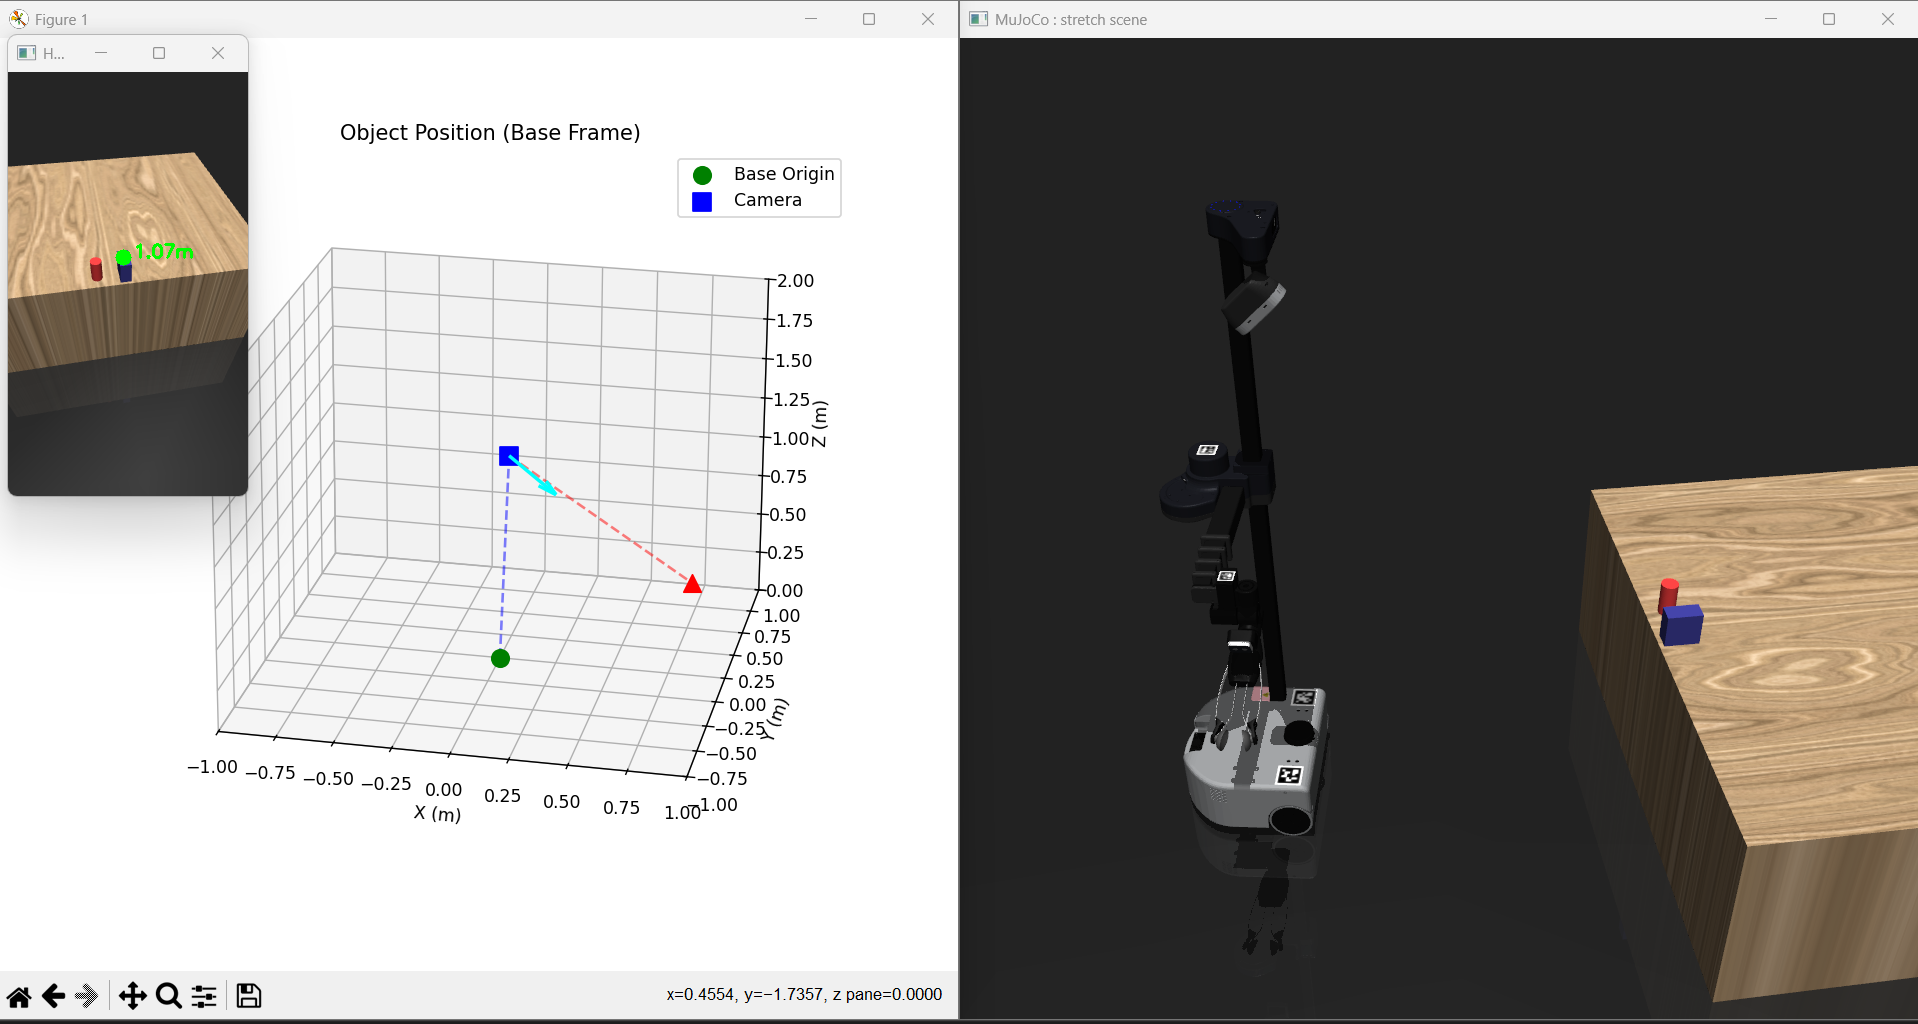
\includegraphics[width=0.85\textwidth]{p4_1_object_detected_and_plotter.png}
    \caption{Left: Head RGB camera with green centroid dot and depth label. Right: 3D plotter showing camera frustum (blue cone) and object position (red dot) in the robot base frame.}
    \label{fig:p4_1}
\end{figure}

\begin{checklistbox}
\begin{itemize}[leftmargin=*]
    \item[\(\square\)] Green dot appears on the blue object in the RGB window
    \item[\(\square\)] Depth label shows a reasonable distance in metres (e.g.\ 0.8m--2.0m)
    \item[\(\square\)] Red dot in the 3D plotter stays approximately fixed when you pan/tilt the head
    \item[\(\square\)] Script exits cleanly with Ctrl+C and both windows close
\end{itemize}
\end{checklistbox}

\begin{warnbox}
If the depth label shows \texttt{None} or the red dot jumps erratically, the object may be at the edge of the depth camera's range, or the object is too small in the frame. Move the object closer (within 1.5\,m) or use a larger object.
\end{warnbox}

\newpage

\section*{Part 2 --- Autonomous Approach}

\subsection*{Objective}

Drive toward the object and stop at $\sim$50\,cm with the object to the robot's right (the ``flank'' position). The wrist camera faces sideways, so presenting the right flank gives it a clear view of the object for the next two phases.

\subsection*{Background: Base-Frame Coordinates}

Extract the object position from \texttt{obj2base\_T[0:3, 3]} as \texttt{x, y, z}. In the robot base frame: $+x$ is ahead, $+y$ is left, $+z$ is up. The horizontal angle to the object is $\theta = \text{atan2}(y, x)$, where $\theta = 0$ is straight ahead and $\theta = -\pi/2$ is directly to the right.

\subsection*{Task}

Copy \texttt{p4\_1\_locate\_object.py} to \texttt{p4\_2\_approach.py}. Remove the \texttt{ObjectPlotter} import and construction---you no longer need the 3D visualization. Add \texttt{StateController} and \texttt{math} to your imports.

Declare all tuning constants at the top of \texttt{main()}, before the loop:

\begin{lstlisting}[language=Python]
Kp_pan     = 1.0
Kp_tilt    = 1.0
Kp_angle   = 5.0 / math.pi
Kp_forward = 2.0
Kp_lift    = 5.0
\end{lstlisting}

Also declare the hysteresis state variable before the loop:

\begin{lstlisting}[language=Python]
in_zone = False
\end{lstlisting}

\subsubsection*{Step 1: Stow Pose --- Keep the Arm Safe While Driving}

Create a \texttt{StateController} that holds the arm retracted and the gripper in a safe position while the robot drives. If the arm is extended during base motion, it could collide with the environment:

\begin{lstlisting}[language=Python]
stow_pose = StateController(controller, {
    "wrist_roll_counterclockwise": 0.0,
    "wrist_yaw_counterclockwise": 0.0,
    "wrist_pitch_up": 0.0,
    "gripper_open": 0.3,
    "arm_out": 0.0,
})
\end{lstlisting}

At the \emph{end} of the loop (after your logic), merge this into the velocities:

\begin{lstlisting}[language=Python]
velocities = merge_proportional(velocities, stow_pose.get_command())
\end{lstlisting}

\subsubsection*{Step 2: Head Tracking --- Keep the Object in View}

Inside the centroid-found block, servo the head to keep the object centered in the frame. Compute normalized pixel errors (in the range $-0.5$ to $+0.5$) and apply proportional control:

\begin{lstlisting}[language=Python]
cx, cy = centroid
frame_cx = rgb.shape[1] / 2
frame_cy = rgb.shape[0] / 2

error_x = (cx - frame_cx) / rgb.shape[1]
error_y = (cy - frame_cy) / rgb.shape[0]
auto_velocities["head_pan_counterclockwise"] = -Kp_pan * error_x
auto_velocities["head_tilt_up"]              = -Kp_tilt * error_y
\end{lstlisting}

\subsubsection*{Step 3: Localize and Compute Angle/Distance}

Directly after head tracking, call \texttt{locate\_object} with the head camera and extract position:

\begin{lstlisting}[language=Python]
_, obj2base_T = locate_object((cx, cy), HEAD_CAMERA, transforms)
if obj2base_T is not None:
    x, y, z = obj2base_T[0:3, 3]
    angle_z            = math.atan2(y, x)
    horizontal_distance = math.sqrt(x**2 + y**2)
\end{lstlisting}

All of the base motion logic (Steps 4--6 below) goes inside this \texttt{if obj2base\_T is not None:} block.

\subsubsection*{Step 4: Base Rotation and Gated Forward Motion}

Rotate the base toward the object and drive forward---but only when well-aligned (within $\sim$18°) to avoid driving sideways:

\begin{lstlisting}[language=Python]
auto_velocities["base_counterclockwise"] = -Kp_angle * angle_z
\end{lstlisting}

Moving forward when badly misaligned is dangerous---the robot might drive sideways. Gate forward motion on alignment by computing how well-aligned the robot is and only allowing forward speed in the last 10\% of perfect alignment:

\begin{lstlisting}[language=Python]
alignment   = 1.0 - abs(angle_z) / math.pi   # 1.0 = facing it, 0.0 = 180 deg away
travel_auth = max(0.0, min(1.0, (alignment - 0.9) / 0.1))
auto_velocities["base_forward"] = Kp_forward * horizontal_distance * travel_auth
\end{lstlisting}

\begin{notebox}
\texttt{travel\_auth} is 0 unless \texttt{alignment > 0.9}, meaning the robot must be within about 18° of facing the object before it will drive forward. This prevents the robot from driving sideways while turning.
\end{notebox}

\subsubsection*{Step 5: Flank Presentation with Hysteresis}

When within 45--55\,cm, stop advancing and rotate to the right flank. The \texttt{in\_zone} flag prevents oscillation: the robot must drift outside 40--60\,cm to exit flank mode:

\begin{lstlisting}[language=Python]
# Update zone membership with hysteresis
if not in_zone:
    if 0.45 <= horizontal_distance <= 0.55:
        in_zone = True
else:
    if horizontal_distance < 0.4 or horizontal_distance > 0.6:
        in_zone = False

# Choose behavior based on zone
if in_zone:
    # Rotate to flank angle (-pi/2 = object to the right)
    angle_error = -math.pi / 2 - angle_z
    auto_velocities["base_counterclockwise"] = Kp_angle * angle_error
    auto_velocities["base_forward"] = 0.0
    print(f"\rDist: {horizontal_distance:.2f}m  "
          f"Angle Err: {math.degrees(angle_error):+6.1f}deg  [FLANK]   ",
          end="", flush=True)
else:
    # Face and drive toward object (code from Step 4)
    auto_velocities["base_counterclockwise"] = -Kp_angle * angle_z
    alignment   = 1.0 - abs(angle_z) / math.pi
    travel_auth = max(0.0, min(1.0, (alignment - 0.9) / 0.1))
    auto_velocities["base_forward"] = Kp_forward * horizontal_distance * travel_auth
    print(f"\rDist: {horizontal_distance:.2f}m  "
          f"Align: {alignment:.3f}  Auth: {travel_auth:.2f}  [moving]   ",
          end="", flush=True)
\end{lstlisting}

\subsubsection*{Step 6: Lift Pre-positioning}

Start raising the lift during approach so it's already at the right height when flanked. The \texttt{+0.10} offset targets 10\,cm above the object, leaving room to descend during alignment:

\begin{lstlisting}[language=Python]
cam_z = transforms.get_wrist_cam_T()[2, 3]
auto_velocities["lift_up"] = Kp_lift * (z - (cam_z + 0.01) + 0.10)
\end{lstlisting}

\subsection*{Expected Result}

Place a blue object at table height in front of the robot and run:

\begin{lstlisting}[language=bash]
uv run p4_2_approach.py
\end{lstlisting}

Watch the terminal output. You should see the \texttt{[moving]} state as the robot drives toward the object, then the \texttt{[FLANK]} state as it rotates. The robot should come to rest with the object approximately to its right.

\begin{figure}[H]
    \centering
    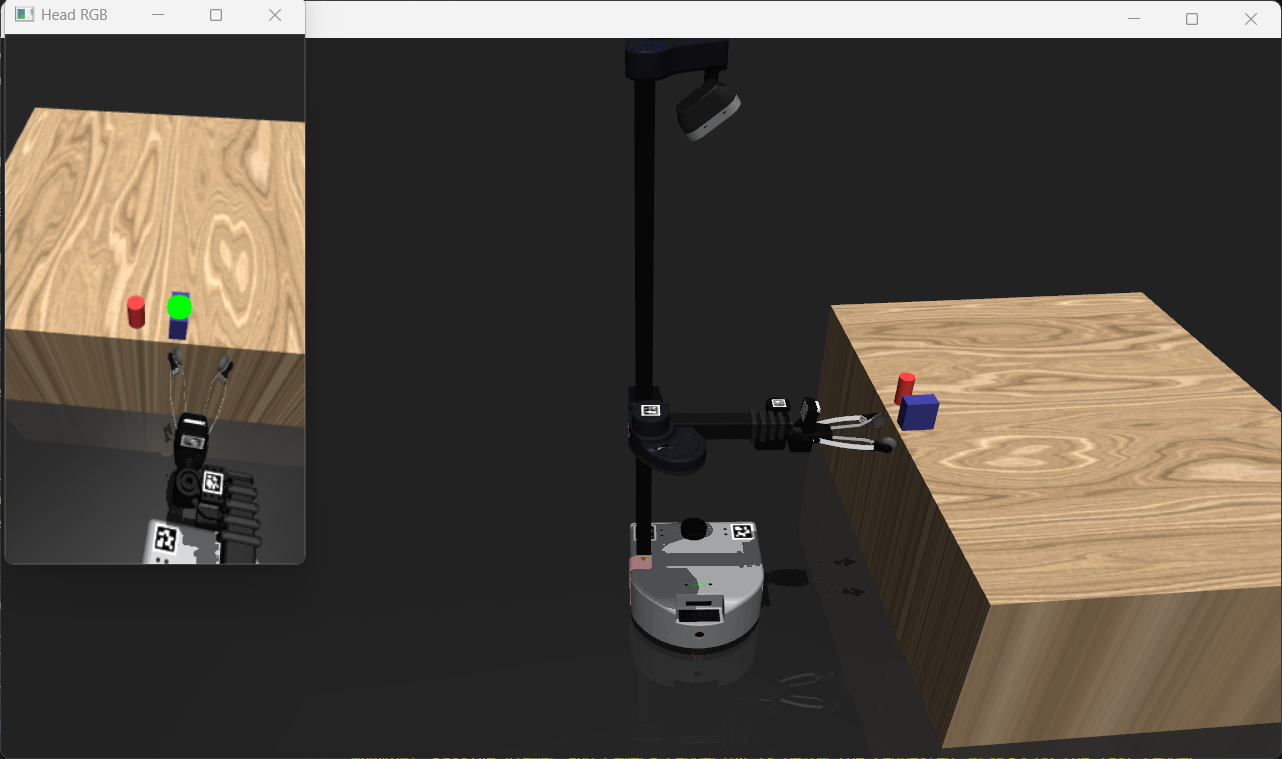
\includegraphics[width=0.85\textwidth]{p4_2_flank_position_achieved.png}
    \caption{Robot in flank position with the blue object to its right. Terminal shows \texttt{[FLANK]} with a small angle error.}
    \label{fig:p4_2}
\end{figure}

\begin{checklistbox}
\begin{itemize}[leftmargin=*]
    \item[\(\square\)] Terminal shows \texttt{[moving]} while the robot drives toward the object
    \item[\(\square\)] Terminal switches to \texttt{[FLANK]} when the robot is within 45--55\,cm
    \item[\(\square\)] The angle error printed in \texttt{[FLANK]} mode approaches $0°$ as the robot rotates
    \item[\(\square\)] The lift rises during approach (the arm moves upward)
    \item[\(\square\)] The arm stays retracted (\texttt{arm\_out = 0}) throughout
\end{itemize}
\end{checklistbox}

\begin{warnbox}
If the robot drives past the object without entering flank mode, the object may be too high or far away for the depth reading to be reliable. Try placing the object within 1.5\,m and ensuring it is clearly visible from the starting position.
\end{warnbox}

\newpage

\section*{Part 3 --- Fine Alignment}

\subsection*{Objective}

The approach phase gets the robot roughly into position, but small angle and height errors remain. This phase switches to the wrist camera---mounted near the gripper---to fine-tune base rotation and lift height until the gripper is precisely lined up.

\subsection*{Task}

Copy \texttt{p4\_2\_approach.py} to \texttt{p4\_3\_align.py}. Add \texttt{WRIST\_CAMERA} and \texttt{WRIST\_RGB\_CAMERA} to your imports from \texttt{stretch\_toolkit}.

\subsubsection*{Step 1: Add Phase State Variable}

Before the loop (alongside \texttt{in\_zone}), add:

\begin{lstlisting}[language=Python]
phase = "approach"
print(f"Phase: {phase}")
\end{lstlisting}

\subsubsection*{Step 2: Wrap Approach Logic in a Phase Check}

Wrap your existing approach block in \texttt{if phase == "approach":}. Nothing inside it changes---you are just gating it:

\begin{lstlisting}[language=Python]
if phase == "approach":
    # ... everything from Part 2 ...
\end{lstlisting}

\subsubsection*{Step 3: Add the Approach-to-Align Transition}

Inside the \texttt{in\_zone} branch of the approach logic, after the print statement, add a transition condition. When the flank angle error is small enough, the robot is correctly oriented---switch to the align phase and close the head camera window:

\begin{lstlisting}[language=Python]
if in_zone:
    angle_error = -math.pi / 2 - angle_z
    auto_velocities["base_counterclockwise"] = Kp_angle * angle_error
    auto_velocities["base_forward"] = 0.0
    print(f"\rDist: {horizontal_distance:.2f}m  "
          f"Angle Err: {math.degrees(angle_error):+6.1f}deg  [FLANK]   ",
          end="", flush=True)
    # Transition to align once roughly flanked
    if abs(angle_error) < math.radians(5):
        cv2.destroyWindow("Head RGB")
        phase = "align"
        print(f"\nPhase: {phase}")
\end{lstlisting}

\subsubsection*{Step 4: Add the Align Phase}

After the approach block, add:

\begin{lstlisting}[language=Python]
elif phase == "align":
    rgb = WRIST_RGB_CAMERA.get_frame()
    centroid = find_blue_object(rgb)

    if centroid is not None:
        cx, cy = centroid
        _, obj2base_T = locate_object((cx, cy), WRIST_CAMERA, transforms)
        if obj2base_T is not None:
            x, y, z = obj2base_T[0:3, 3]
            angle_z = math.atan2(y, x)
            cam_z   = transforms.get_wrist_cam_T()[2, 3]

            # Rotate base toward final flank target (3 deg bias for gripper offset)
            auto_velocities["base_counterclockwise"] = \
                Kp_angle * (-math.pi / 2 - angle_z + math.radians(3))
            # Move lift until object is level with wrist camera
            auto_velocities["lift_up"] = Kp_lift * (z - (cam_z + 0.01))

            # Check transition conditions
            angle_err = abs(-math.pi / 2 - angle_z)
            lift_err  = abs(z - (cam_z + 0.01))
            if stow_pose.is_at_goal() and \
               angle_err < math.radians(5) and \
               lift_err < 0.03:
                phase = "done"
                print(f"\nPhase: {phase}")

        if rgb is not None:
            cv2.circle(rgb, (cx, cy), 10, (0, 255, 0), -1)

    if rgb is not None:
        cv2.imshow("Wrist RGB", rgb)

    velocities = merge_proportional(velocities, auto_velocities)
    velocities = merge_proportional(velocities, stow_pose.get_command())
\end{lstlisting}

\begin{notebox}
The \texttt{3°} bias (\texttt{math.radians(3)}) in the base rotation command compensates for the physical offset between the wrist camera lens and the gripper fingertips. Without it, the camera would be centered on the object but the gripper would be slightly off to one side.
\end{notebox}

\subsubsection*{Step 5: Add the Done Phase}

The \texttt{"done"} phase simply holds the robot in place (no commands). Add it after the align block:

\begin{lstlisting}[language=Python]
elif phase == "done":
    pass  # Hold position
\end{lstlisting}



\subsection*{Expected Result}

\begin{lstlisting}[language=bash]
uv run p4_3_align.py
\end{lstlisting}

The approach phase runs as before. When the flank angle is achieved, the \texttt{Head RGB} window closes, the \texttt{Wrist RGB} window opens, and the terminal prints \texttt{Phase: align}. The robot makes small adjustments to rotation and lift. When all three conditions are met, it prints \texttt{Phase: done} and holds.

\begin{figure}[H]
    \centering
    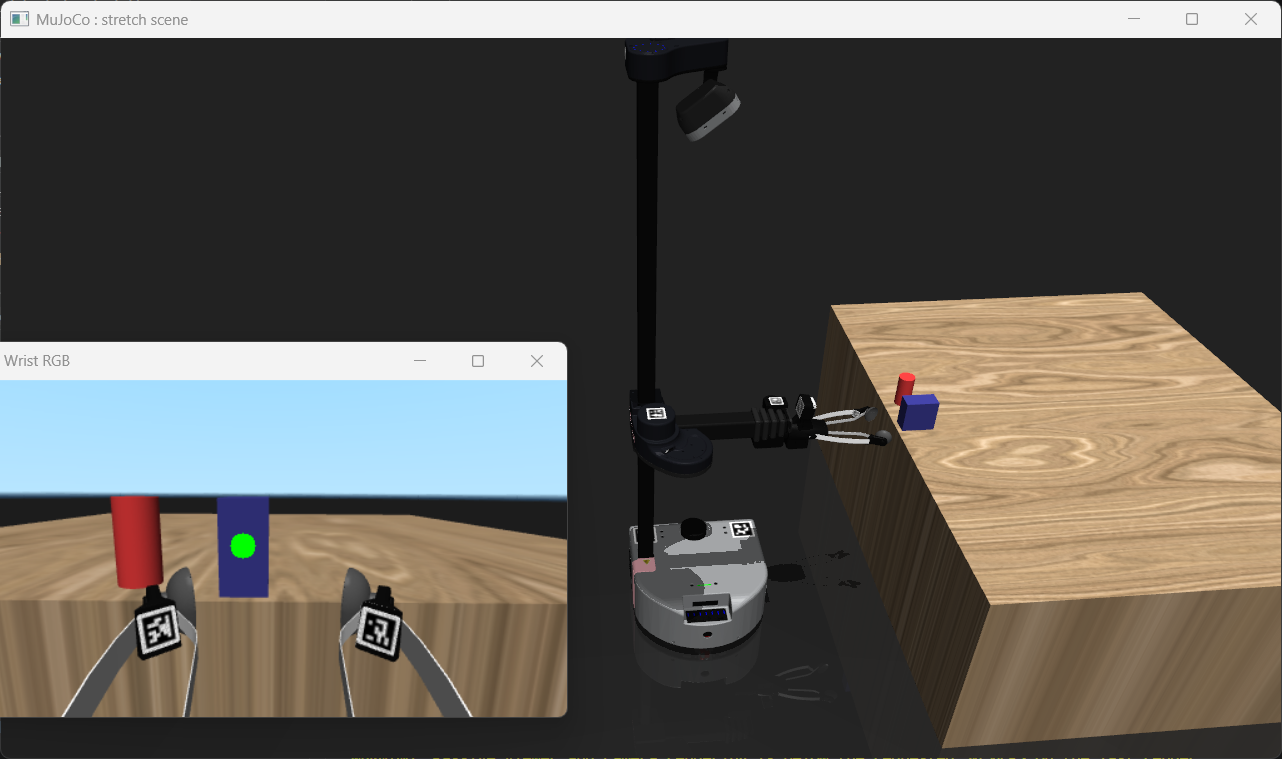
\includegraphics[width=0.85\textwidth]{p4_3_wrist_camera_aligned.png}
    \caption{Wrist RGB camera view during the align phase. The blue object's centroid (green dot) is approximately centered in the frame, indicating the robot is ready to reach.}
    \label{fig:p4_3}
\end{figure}

\begin{checklistbox}
\begin{itemize}[leftmargin=*]
    \item[\(\square\)] Terminal prints \texttt{Phase: align} after the head window closes
    \item[\(\square\)] The wrist camera window opens and shows the blue object
    \item[\(\square\)] The robot makes small adjustments (not large oscillations)
    \item[\(\square\)] Terminal eventually prints \texttt{Phase: done} and the robot stops
\end{itemize}
\end{checklistbox}

\begin{warnbox}
If the align phase never transitions to \texttt{"done"}, the most common cause is that \texttt{stow\_pose.is\_at\_goal()} is never \texttt{True}. Verify that you are calling \texttt{merge\_proportional(velocities, stow\_pose.get\_command())} at the end of the align block---if the stow pose commands are not being sent, the joints never reach their targets.
\end{warnbox}

\newpage

\section*{Part 4 --- Arm Extension and Wrist Servoing}

\subsection*{Objective}

Extend the arm while using the wrist camera to keep the object centered. The arm stops at 12\,cm depth---the point where the gripper fingers reach the object.

\subsection*{Task}

Copy \texttt{p4\_3\_align.py} to \texttt{p4\_4\_reach.py}.

\subsubsection*{Step 1: Add Tuning Constants}

Add these constants alongside the others at the top of \texttt{main()}:

\begin{lstlisting}[language=Python]
Kp_yaw   = 0.5
Kp_pitch = 0.5
Kp_arm   = 10.0
\end{lstlisting}

\subsubsection*{Step 2: Add the Pre-Grip Pose Controller}

Add a second \texttt{StateController} for use during the reach phase. This opens the gripper slightly and straightens the wrist roll, so the gripper arrives at a good orientation:

\begin{lstlisting}[language=Python]
pre_grip_pose = StateController(controller, {
    "wrist_roll_counterclockwise": 0.0,
    "gripper_open": 0.4,
})
\end{lstlisting}

\subsubsection*{Step 3: Change the Align Transition Target}

In the align block, change:
\begin{lstlisting}[language=Python]
phase = "done"
\end{lstlisting}
to:
\begin{lstlisting}[language=Python]
phase = "reach"
\end{lstlisting}

\subsubsection*{Step 4: Add the Reach Phase}

After the align block and before the done block, add:

\begin{lstlisting}[language=Python]
elif phase == "reach":
    rgb = WRIST_RGB_CAMERA.get_frame()
    centroid = find_blue_object(rgb)

    if centroid is not None:
        cx, cy = centroid

        # Servo wrist to keep object centered
        if rgb is not None:
            frame_cx = rgb.shape[1] / 2
            frame_cy = rgb.shape[0] / 2
            error_x = (cx - frame_cx) / rgb.shape[1]
            error_y = (cy - frame_cy) / rgb.shape[0]
            auto_velocities["wrist_yaw_counterclockwise"] = Kp_yaw * error_x
            auto_velocities["wrist_pitch_up"]             = -Kp_pitch * error_y
            cv2.circle(rgb, (cx, cy), 10, (0, 255, 0), -1)

        # Extend arm based on depth
        distance = WRIST_CAMERA.get_depth((cx, cy))
        if distance is not None:
            distance_error = distance - 0.12
            auto_velocities["arm_out"] = Kp_arm * distance_error
            print(f"\rDepth: {distance:.3f}m  Error: {distance_error:+.3f}m   ",
                  end="", flush=True)
            if abs(distance_error) < 0.02 and pre_grip_pose.is_at_goal():
                phase = "done"
                print(f"\nPhase: {phase}")

    if rgb is not None:
        cv2.imshow("Wrist RGB", rgb)

    velocities = merge_proportional(velocities, auto_velocities)
    velocities = merge_proportional(velocities, pre_grip_pose.get_command())
\end{lstlisting}

\begin{notebox}
Notice that the reach phase uses \texttt{pre\_grip\_pose.get\_command()} instead of \texttt{stow\_pose.get\_command()}. This is critical: \texttt{stow\_pose} would command \texttt{arm\_out = 0} which would fight against the arm extension. Switch to \texttt{pre\_grip\_pose} which does not constrain the arm.
\end{notebox}

\subsection*{Expected Result}

\begin{lstlisting}[language=bash]
uv run p4_4_reach.py
\end{lstlisting}

After alignment, the arm should extend toward the object. The terminal will print live depth readings. When the object is 12\,cm away and the gripper pose is stable, the script prints \texttt{Phase: done} and holds.

\begin{figure}[H]
    \centering
    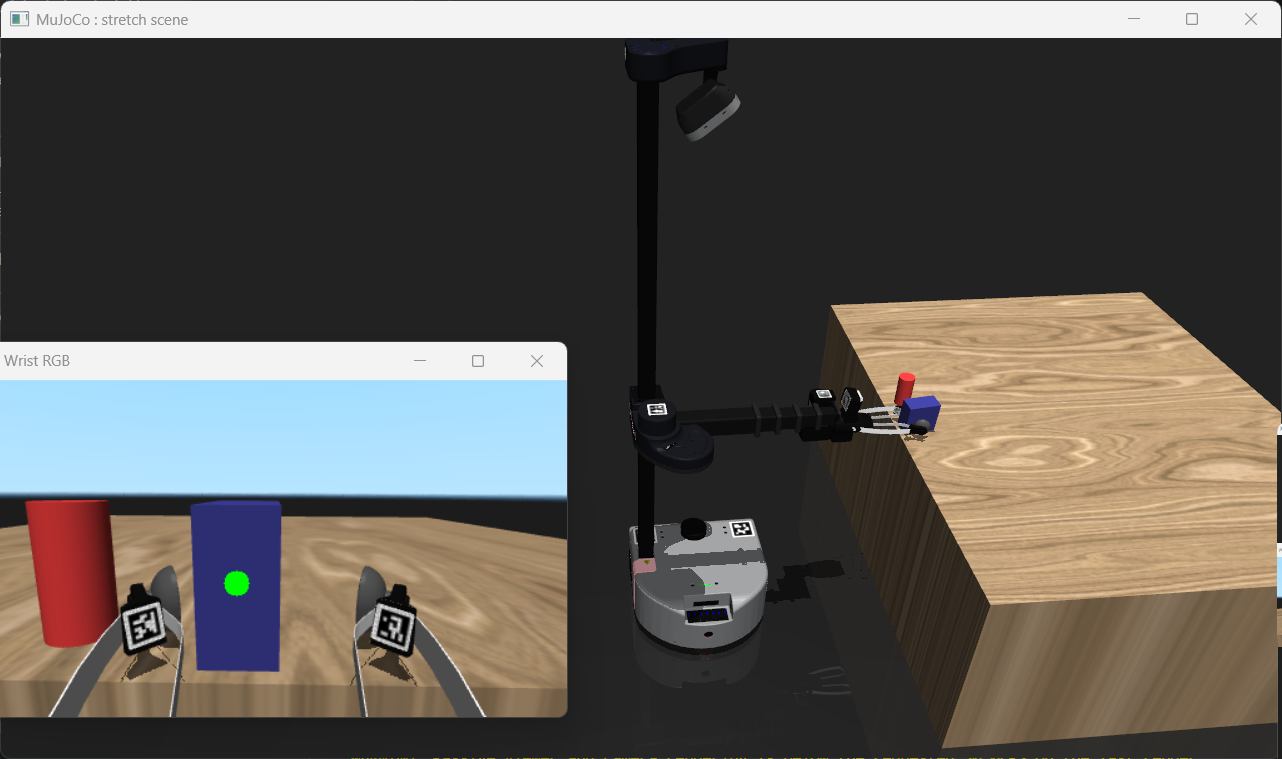
\includegraphics[width=0.85\textwidth]{p4_4_arm_extended_close_to_object.png}
    \caption{Wrist camera view with the arm extended. The blue object fills more of the frame as the arm approaches. Terminal shows depth decreasing toward 0.12\,m.}
    \label{fig:p4_4}
\end{figure}

\begin{checklistbox}
\begin{itemize}[leftmargin=*]
    \item[\(\square\)] Arm extends after alignment (not before)
    \item[\(\square\)] Terminal shows decreasing depth values as the arm extends
    \item[\(\square\)] Depth stabilizes near 0.12\,m (12\,cm)
    \item[\(\square\)] Terminal prints \texttt{Phase: done} when depth is within 2\,cm of 0.12\,m
\end{itemize}
\end{checklistbox}

\begin{warnbox}
If the arm oscillates (extends and retracts repeatedly without settling), the gain \texttt{Kp\_arm = 10.0} may be too high. Reduce it to \texttt{5.0} if this occurs. If the arm extends but depth never reaches 0.12\,m, the object may be out of the arm's reach---try repositioning it closer to the robot.
\end{warnbox}

\newpage

\section*{Part 5 --- Grab}

\subsection*{Objective}

Close the gripper and lift the arm to complete the pick.

\subsection*{Task}

Copy \texttt{p4\_4\_reach.py} to \texttt{p4\_5\_grab.py}.

\subsubsection*{Step 1: Change the Reach Transition Target}

In the reach block, change:
\begin{lstlisting}[language=Python]
phase = "done"
\end{lstlisting}
to:
\begin{lstlisting}[language=Python]
phase = "grab"
\end{lstlisting}

\subsubsection*{Step 2: Add the Grab Phase}

After the reach block, add:

\begin{lstlisting}[language=Python]
elif phase == "grab":
    auto_velocities["lift_up"]      = 0.2
    auto_velocities["gripper_open"] = -1.0
    velocities = merge_proportional(velocities, auto_velocities)
\end{lstlisting}

This phase runs indefinitely until you terminate with Ctrl+C.

\begin{notebox}
Do not call \texttt{stow\_pose.get\_command()} or \texttt{pre\_grip\_pose.get\_command()} in the grab phase. Both would counteract the gripper close command (\texttt{stow\_pose} targets \texttt{gripper\_open = 0.3}; the grab phase needs \texttt{gripper\_open = -1.0}).
\end{notebox}

\subsection*{The Complete Pipeline}

Your \texttt{p4\_5\_grab.py} implements the full autonomous pick sequence:

\begin{enumerate}
    \item \textbf{Approach} --- Head camera tracks object; base drives forward with alignment gating; flank presentation at 50\,cm; lift pre-positions 10\,cm above target.
    \item \textbf{Align} --- Wrist camera fine-tunes base rotation and lift until all three conditions are met.
    \item \textbf{Reach} --- Arm extends toward object; wrist servos re-center continuously; transition at 12\,cm depth.
    \item \textbf{Grab} --- Gripper closes; lift rises.
\end{enumerate}

\subsection*{Expected Result}

Place a blue object at table height and run:

\begin{lstlisting}[language=bash]
uv run p4_5_grab.py
\end{lstlisting}

The terminal should print each phase transition:

\begin{lstlisting}
Phase: approach
Phase: align
Phase: reach
Phase: grab
\end{lstlisting}

The robot should complete the full sequence and lift the object.

\begin{figure}[H]
    \centering
    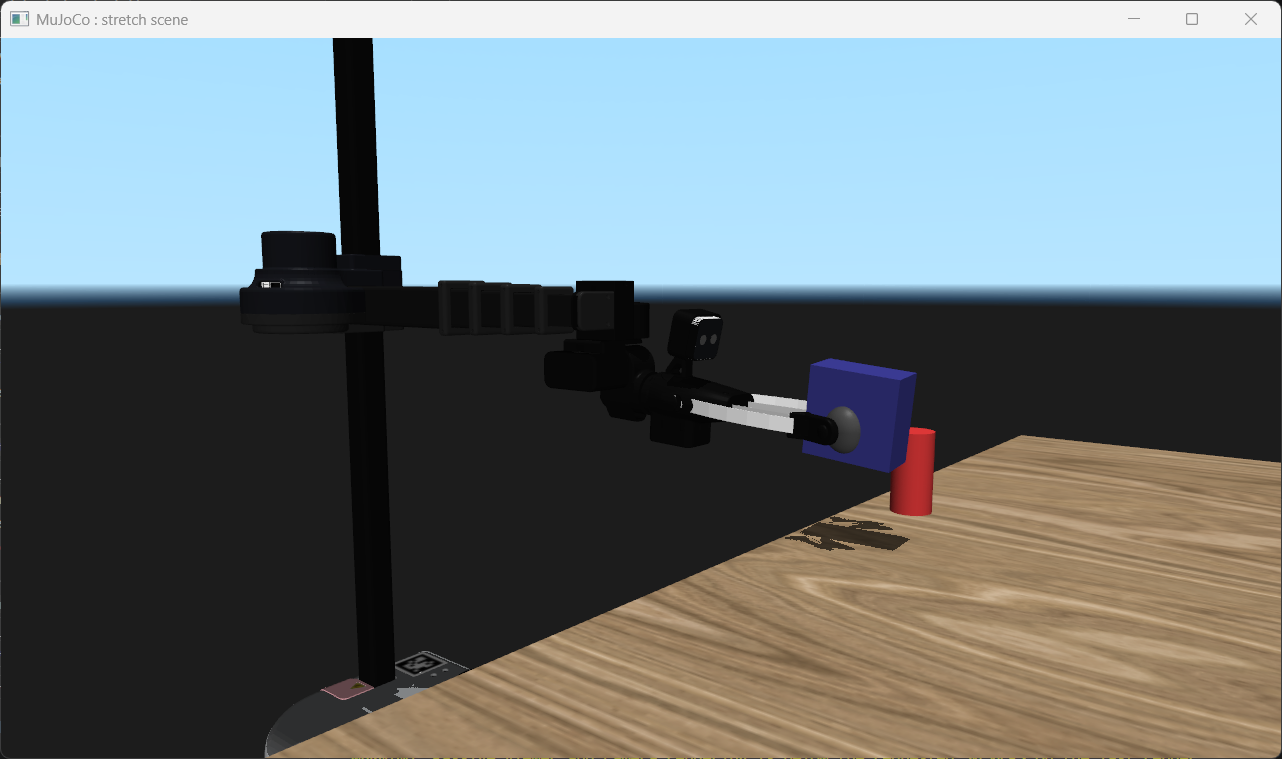
\includegraphics[width=0.85\textwidth]{p4_5_gripper_closed_object_lifted.png}
    \caption{Robot completing the grab: gripper closed around the blue object with the lift raised. Terminal shows all four phase transitions.}
    \label{fig:p4_5}
\end{figure}

\begin{checklistbox}
\begin{itemize}[leftmargin=*]
    \item[\(\square\)] All four phase transitions print in order
    \item[\(\square\)] Gripper closes in the grab phase
    \item[\(\square\)] Lift raises after gripper closes
    \item[\(\square\)] The script exits cleanly with Ctrl+C
\end{itemize}
\end{checklistbox}

\begin{warnbox}
If the gripper closes but doesn't lift the object (it slides through), the align or reach phases may have left the gripper slightly off-center. Run Part 3 or Part 4 in isolation and observe the wrist camera view to check alignment before attempting the full pipeline.
\end{warnbox}

\newpage

\section*{Deliverable}

Record a screen capture with voiceover demonstrating your complete system running \texttt{p4\_5\_grab.py} on the simulator. The recording should show the robot completing the full pick without any manual intervention.

\subsection*{Required Content}

Your video must include:

\begin{enumerate}
    \item \textbf{All four phase transitions} visible in the terminal output
    \item \textbf{Approach phase}: the robot driving toward the object, switching to \texttt{[FLANK]} mode in the terminal
    \item \textbf{Align phase}: the wrist camera window opening and the robot making small adjustments
    \item \textbf{Reach phase}: the arm extending and the depth reading decreasing toward 12\,cm in the terminal
    \item \textbf{Grab phase}: the gripper closing and the lift raising the object
\end{enumerate}

\subsection*{Voiceover}

In your voiceover, address the following:

\begin{itemize}
    \item How does the robot determine where the object is in 3D space? (Mention forward kinematics and the depth camera.)
    \item Why does the robot present its flank instead of approaching directly?
    \item Why are there three separate conditions required to transition from align to reach?
    \item Describe \emph{one change} you would make to the pipeline to make it more robust or reliable.
\end{itemize}

\end{document}
